\documentclass[12pt]{extarticle}
\usepackage[utf8]{inputenc}
\usepackage[english]{babel}
\usepackage{amsmath}
\usepackage{amsfonts}
\usepackage{amssymb}
\usepackage[margin=12mm,includefoot]{geometry}
\usepackage[hidelinks]{hyperref}

%Header and Footer Stuff
\usepackage{fancyhdr} 
\pagestyle{fancy}
\fancyhead{}
\cfoot{}
\rfoot{\thepage}
\renewcommand{\headrulewidth}{0pt}
\renewcommand{\footrulewidth}{0.1mm}

%Bullet
\renewcommand{\labelitemi}{-}
\renewcommand{\labelitemii}{$\circ$}
\renewcommand{\labelitemiii}{}

%Image
\usepackage{graphicx}
\usepackage{float}
\usepackage{caption}
\usepackage{subcaption}

%Tree
\usepackage{forest}

%Style Section
\usepackage[explicit]{titlesec}

\titleformat{\section}
  {\normalfont\Large\bfseries}{\thesection}{1em}{\MakeUppercase{#1}}	
  
%FrameBox
\usepackage[usestackEOL]{stackengine}

%Table
\usepackage{multirow}
\setlength{\tabcolsep}{0.5em} % for the horizontal padding
\renewcommand{\arraystretch}{1.2}% for the vertical padding


\date{}
\author{Francesco Buttafuoco}


\newcommand{\hmwkTitle}{Synthesis and optimization of digital systems} % Assignment title
\newcommand{\hmwkDueDate}{2015/2016} % Due date
\newcommand{\spaceBreackLine}{3mm} 

\title{
\vspace{2in}
\textmd{\textbf{\hmwkTitle}}\\
\normalsize\vspace{0.1in}\normalsize{\hmwkDueDate}\\
\vspace{3in}
}


\begin{document}

\maketitle
\thispagestyle{empty}
\newpage

\tableofcontents	

\thispagestyle{empty}
\cleardoublepage
\setcounter{page}{1}


\section{Introduction}

\subsection{Microelectronic Economics}
\begin{itemize}
\item \textbf{Fixed Costs}: Design
\item \textbf{Variable Costs}: Energy for manufacturing, material needed
\end{itemize}
The higher the integration level, the better and cheaper the final product, true for high-volume production. In fact volume recaptures manufacturing and designs cost.
\bigskip \\
For applications that do not enjoy high-volume (ASICs), other factors matter: reduction of design time (and cost) and quality of the design.
\bigskip \\
\textbf{Variability}: variation of the geometry of transistor that introduce error about speed because \textit{lithography} is not so precise and do not allow to create a good channel in the transistors.

\subsection{CAD}
\textbf{CAD} (Computer-Aided Design) allow to:
\begin{itemize}
\item Reduces design time
\item Multi-objective optimization (area, speed, power)
\item Large scale design management
\end{itemize}
CAD tools reduce time to market, reducing the \textit{fixed cost}. Moreover you can also reduce the \textit{variable cost} optimizing the area and using less silicon.

\subsection{Integrated Circuit Design Styles}
\begin{figure}[H]
	\centering
	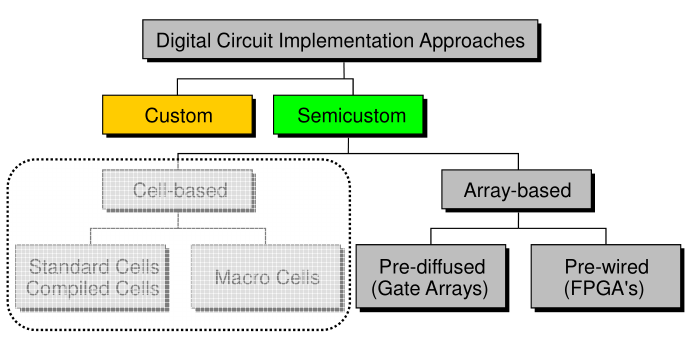
\includegraphics[height=90 mm]{./Cap1/Images/Image01.png}
	\caption[Optional caption]{Integrated Circuit Design Styles}
	\label{fig:ICDS}
\end{figure}
The \textbf{custom} approach (design \textit{by hand}):
\begin{itemize}
\item Functional and physical design are hand-crafted operations
\item Extensive effort (and cost) to optimize each feature
\item Typical of \textit{critical portions} of high-performance designs
\end{itemize}
The \textbf{Semi-custom} approaches
\begin{itemize}
\item Limited number of circuits primitives that allows designers to leverage “optimized” primitives and focus on their \textit{interconnection}
\item Semi-custom design are the big majority of digital design
\end{itemize}
Type of \textbf{Semi-custom} approaches:
\begin{itemize}
\item \textbf{Cell-based}: use  standard cells  or  macrocells  (larger functions)
\begin{itemize}
\item \textbf{Standard cells}: Designed once and highly optimized, stored into a library
\item  \textbf{Macrocells}: Primitives generated by  module generators, ynthesized layout thanks to predefined structures (SRAMs, ROMs)
\end{itemize}
\item \textbf{Array-based}:  Exploit the use of a matrix of uncommitted components which are eventually personalized and connected
\begin{itemize}
\item \textbf{Re-diffused arrays}: Personalization by metalization/contacts (MPGAs).
\item \textbf{Pre-wired arrays}: Personalization on the field (FPGAs).
\end{itemize}
\end{itemize}

\subsection{Microelectronic Design}
Three major tasks (repeated at different \textit{Abstraction levels}):
\begin{itemize}
\item \textbf{Conceptualization and modeling} (Description): Hardware Description Languages (HDL)
\item \textbf{Synthesis and optimization}: Create the structure
\item \textbf{Validation}: Check for correctness
\end{itemize}
\textbf{Models} can be classified in terms of
\begin{itemize}
\item \textit{Abstraction levels}
\begin{itemize}
\item \textbf{Architectural-level} (or RT-level): Operations implemented by
resources.
\item \textbf{Logic-level}: Logic functions implemented by gates.
\item \textbf{Geometrical-level} (or Circuit-level): Circuit implemented by electronic device
\end{itemize}
\item \textit{Views}
\begin{itemize}
\item \textbf{Behavioral} view: Abstract function.
\item \textbf{Structural} view: An interconnection of parts.
\item \textbf{Physical} view: Physical objects with size and positions.
\end{itemize}
\end{itemize}
\begin{figure}[H]
	\centering
	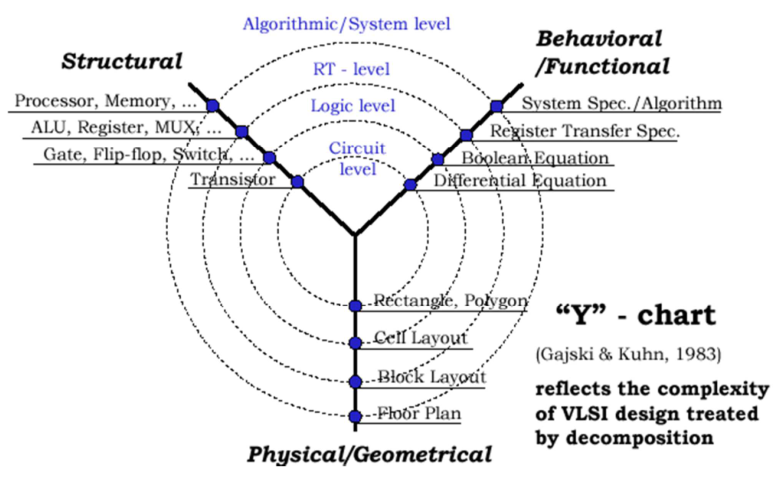
\includegraphics[height=90 mm]{./Cap1/Images/Image02.png}
	\caption[Optional caption]{Y chart}
	\label{fig:Ychart}
\end{figure}
In the Figure \ref{fig:Ychart} the axis represent the \textit{Abstraction levels}, the circles the \textit{Views}.\\
It shows the same \textit{Abstraction levels} at different \textit{Views} and vice versa.\\
The \textbf{synthesis} is the switching from Behavioural to Structural at different \textit{Abstraction levels} and Optimization.\\
Objectives of the Optimization:
\begin{itemize}
\item Area
\item Timing (Performance)
\item Energy consumption
\end{itemize}
Optimization has multiple objectives, it is a trade off.
\begin{figure}[H]
	\centering
	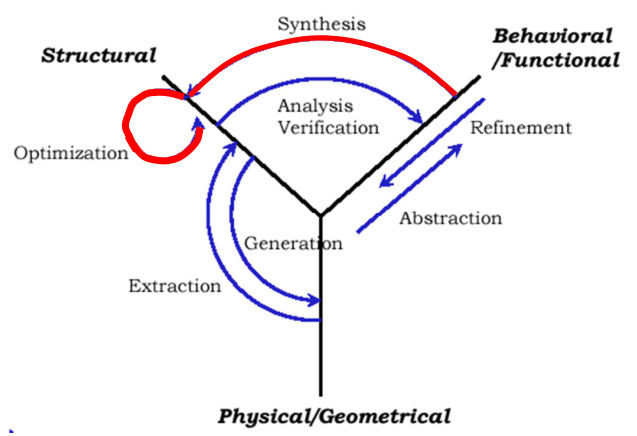
\includegraphics[height=70 mm]{./Cap1/Images/Image03.png}
	\caption[Optional caption]{Synthesis and Optimization}
	\label{fig:SynthOpt}
\end{figure}
\begin{flushleft}
	The \textbf{design} is the repetition of
\end{flushleft}
\begin{enumerate}
\item Modelling
\item Synthesis \& Optimization
\item Validation
\end{enumerate}
for each level: RTL, LOGIC, PHYSICAL.

\subsection{Design space}
The Design Space is where a dimension is a variable. The different feasible structural implementations of a circuit define its design space. The design space is a finite set of design points. Combined optimization of area (minimization) and performance (maximization) can be abstracted by representing the feasible structural implementations of a design into a design space.
\bigskip \\
\textbf{Optimization}: search an implementation that optimizes all
objectives.
\bigskip \\
A  point of the design space is called a  \textbf{Pareto point} if there is no other point (in the design space) with at least an inferior objective, all others being inferior or equal. A Pareto point corresponds to a global optimum in a monodimensional design evaluation space.\\ 
The image of the Pareto points in the design evaluation space is the set of the optimal  trade-off  points. Their interpolation yields a  trade-off curve  or  surface.
\begin{figure}[H]
	\centering
	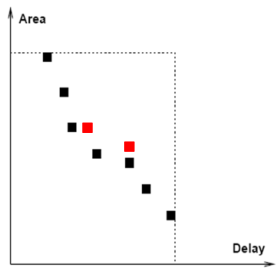
\includegraphics[height=50 mm]{./Cap1/Images/Image04.png}
	\caption[Optional caption]{Pareto Points}
	\label{fig:Pareto}
\end{figure}
\begin{flushleft}
	In the Figure \ref{fig:Pareto} the black points are the Pareto points.
\end{flushleft}

\subsection{General approaches to optimization}
Circuit optimization involves multiple objective functions. The optimization problem is difficult to solve, due to the discontinuous nature of the objective functions and to the discrete nature of the design space, i.e., of the set of feasible circuit implementations. In general, Pareto points  are  solutions to constrained optimization problems.\\
Consider, for example, \textit{logic-level} models. Then the following two problems are of interest:
\begin{itemize}
\item Minimize the circuit  \textit{area}  under  \textit{delay} constraints
\item Minimize the circuit  \textit{delay}  under  \textit{area} constraints
\end{itemize}
Unfortunately, due to the difficulty of the optimization problems, only approximations to the Pareto points can be computed.\\
Consider next \textit{architectural-level} models of synchronous circuits. Pareto points are solutions to the following problems, for different values of the \textbf{cycle-time}:
\begin{itemize}
\item Minimize the circuit \textit{area} under \textit{latency} constraints
\item Minimize the circuit \textit{latency} under \textit{area} constraints
\end{itemize}
These two problems are often referred to as \textit{scheduling problems}.

\cleardoublepage
\section{Modeling Languages and Abstract Models}

\subsection{HDL analysis}
A language can be characterized by its  syntax, semantics  and  pragmatics.\\
The \textit{syntax} relates to the language structure and it can be specified by a grammar.\\
The \textit{semantics} relates to the meaning of a language. The semantic rules associate actions to the language fragments that satisfy the syntax rules.\\
The \textit{pragmatics} relate to the other aspects of the language, including implementation issues. \\
Languages can be broadly classified as  procedural  and  declarative  languages. \textit{Procedural} programs specify the desired action by describing a sequence of steps whose order of execution matters. Conversely, \textit{declarative} models express the problem to be solved by a set of declarations without detailing a solution method. Therefore the order of the statements is not important in such languages.\\
Languages for hardware specification are classified on the basis of the description view that they support (e.g., physical, structural or behavioral).\\
Languages that support \textit{physical design} are characterized by having geometric primitives and by supporting operations on those primitives.\\
Models in \textit{structural languages} describe an interconnection of components. Hence their expressive power is similar to that of circuit schematics, even though specific language constructs can provide more powerful abstractions. Hierarchy is often used to make the description modular and compact.\\
Type of languages:
\begin{itemize}
\item Procedural languages: Specify the action (and so the circuit) by a sequence of steps (C, Pascal, VHDL, Verilog)
\item Declarative languages: Specify the hardware by a set of declaration (Logic netlist, VHDL, Verilog).
\end{itemize}
The success of VHDL and Verilog is due to at behavioral view it possible implement \textit{sequential} and \textit{combinational} descriptions.\\
Models in \textit{behavioral languages} can describe \textit{combinational} or \textit{sequential} circuits.\\
The \textit{combinational} circuit is described as a set of untimed assignment where each assignment represents a virtual logic gate (very similar to procedural models).\\
The sequential circuit is described throw declaration of \textit{Task}, use timing annotation for delayed signals. \\
The \textit{Tasks} can be, at architectural level, generic operations, or, at logic-level, logic functions.

\subsection{Abstract models}
A  model of a circuit is an abstraction, i.e., a representation that shows relevant features without associated details. Formal models have a well-defined syntax and semantics. Hence they provide a way of conveying the information about a circuit in a consistent way that can be unambiguously interpreted. Conversely, informal circuit specifications, such as textual descriptions have limited applications when  CAD  methods are used. In addition, informal descriptions of large-scale circuits or systems may be sources of misunderstanding among humans.\\
A circuit can be modelled differently according to the desired abstraction level (e.g., architectural, logic, geometric), view (e.g., behavioral, structural, physical) and the modelling means (e.g., language, diagram, mathematical model).\\
In recent years, there has been a trend toward using \textbf{hardware description languages} (HDLs) for circuit specification.\\
\textbf{Abstract models} are mathematical models based on graphs and Boolean algebra.\\
At the \textit{architectural level}, the circuit \textit{behavior} can be abstracted by a set of operations (called also tasks) and their dependencies. The operations can be general in nature, ranging from arithmetic to logic functions.\\
At the \textit{logic level}, the \textit{behavior} of a sequential logic circuit is abstracted by a finite-state machine that degenerates to a Boolean function in the  combinational case.\\
\textit{Structural views} are abstracted as interconnections of logic blocks or gates (at the logic level) or resources (at the architectural level).\\
Abstract models are powerful enough to capture the essential features described by HDL and diagram models. 
\begin{figure}[H]
	\centering
	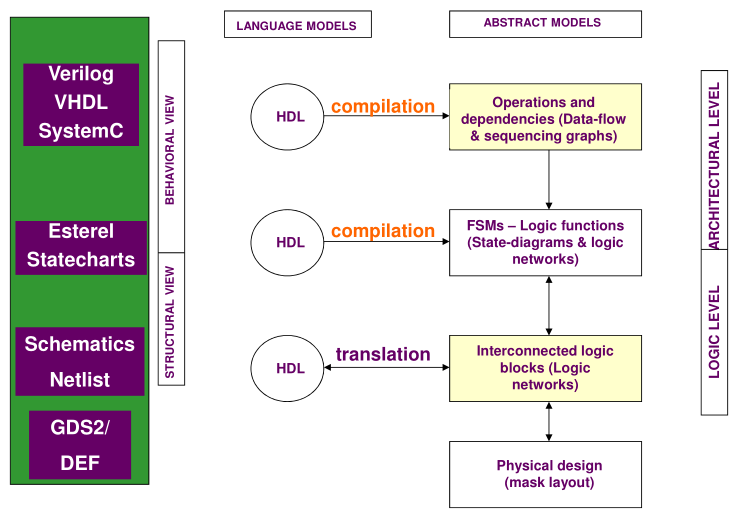
\includegraphics[height=100 mm]{./Cap2/Images/Image01.png}
	\caption[Optional caption]{Languages and abstract models}
	\label{fig:absMod}
\end{figure}
$ $\\[\spaceBreackLine]
Examples of \textbf{Abstract models}
\begin{itemize}
\item \textit{Logic networks}
\begin{itemize}
\item \textit{Mixed structural/behavioral views}
\item \textit{BDD} and \textit{AIG}
\end{itemize}
\item \textit{State diagrams}: The behavioral view of sequential circuits at the logic level can be expressed by finite-state machine transition diagrams
\item \textit{Dataflow} and \textit{sequencing graphs}
\end{itemize}

\subsubsection{Logic network (logic-level)}
A generalized \textit{logic network} is a structure, where each module is associated with a combinational or sequential logic function. Each block is modelled by a Boolean function. Each module is associated with a multiple-input, single-output combinational logic function, called a\textit{ local function}. Pins are partitioned into two classes, called \textit{input} and \textit{outputs}.
\subsubsection{Mixed structural/behavioral views}
In general, a logic network is a hybrid \textit{stmctural/behavioral representation}, because the the interconnections provide a structure while the logic functions denote the terminal behavior of the modules.
\begin{figure}[H]
    \centering
    \begin{subfigure}[b]{0.4\textwidth}
        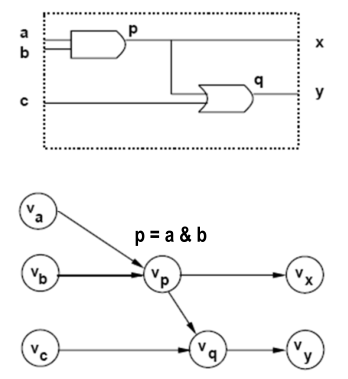
\includegraphics[width=\textwidth]{./Cap2/Images/Image02.png}
        \caption{Mapped network}
        \label{fig:map}
    \end{subfigure}
    \begin{subfigure}[b]{0.4\textwidth}
        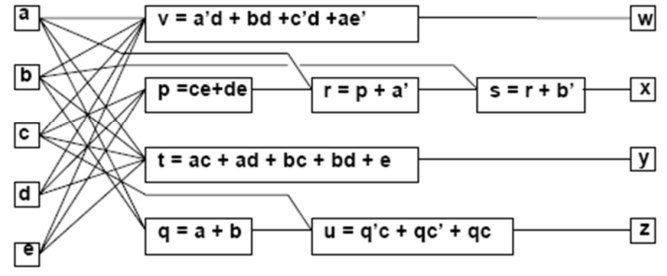
\includegraphics[width=\textwidth]{./Cap2/Images/Image03.png}
        \caption{General network}
        \label{fig:gen}
    \end{subfigure}
    \caption{Different networks}
    \label{fig:nets}
\end{figure}
The Figure \ref{fig:map} is a special case when the blocks correspond to \textit{library elements}.

\subsubsection{BDD (logic-level)}
A Binary Decision Diagram (BDD) is a directed acyclic graph (DAG)
\begin{itemize}
\item \textit{Graph}: set of vertices connected by edges
\item \textit{Directed}: edges have direction
\item \textit{Acyclic}: no path in the graph can lead to a cycle
\end{itemize}
Ordered BDD (\textbf{OBDD}):
\begin{enumerate}
\item Each vertex represents a decision on a variable
\item The value of the function is found at the leaves
\item Each path from root to leaf corresponds to a row in the truth table
\item Variables must appear in the same order along each path from root to leaves
\item Each variable can appear at most once on a path
\end{enumerate}
\begin{figure}[H]
    \centering
    \begin{subfigure}[b]{0.15\textwidth}
        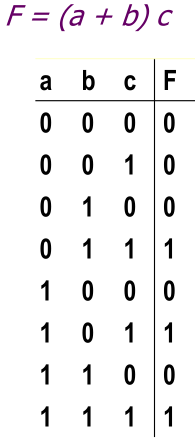
\includegraphics[width=\textwidth]{./Cap2/Images/Image04.png}
        \caption{True Table}
        \label{fig:trueTable}
    \end{subfigure}
    \quad\quad\quad
    \begin{subfigure}[b]{0.4\textwidth}
        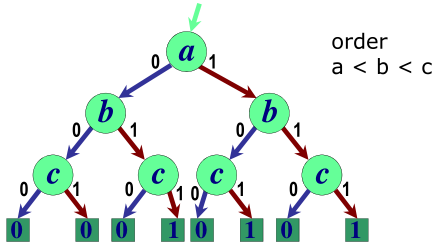
\includegraphics[width=\textwidth]{./Cap2/Images/Image05.png}
        \caption{OBDD}
        \label{fig:OBDD}
    \end{subfigure}
    \label{fig:OBDDs}
\end{figure}
The OBDD is a efficient way to represent logic functions. Each distinct function corresponds to a unique distinct diagram (\textit{Canonical form}). Efficient manipulation of Boolean functions, in fact many logical operations on OBDDs can be implemented in polynomial time (conjunction, negation, disjunction).\\
\textit{Drawbacks}: The size of a BDD is as big as a truth table.
\bigskip \\
The \textbf{Reduced OBDD} is obtained applying 2 roles:
\begin{enumerate}
\item Merging equivalent sub-trees
\item Removing nodes with identical children
\end{enumerate}

\subsubsection{AIG (logic-level)}
An And-Inverter Graph (AIG) is a  directed acyclic graph (DAG).
\textit{Nodes}:
\begin{itemize}
\item Terminal nodes representing variable names
\item Internal nodes representing AND function
\end{itemize}
\textit{Edge}: Those containing markers indicate logical negation.\\
AIG is fast, scalable (less memory) and with efficient manipulation. Each function can have different diagrams, it is not a \textit{Canonical form}.\\
The advantage of the AIG: the number of the leafs is equal to the number of the inputs (n) and not $ 2^{n} $ as in the ROBDD.
\begin{figure}[H]
	\centering
	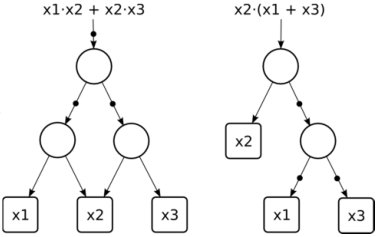
\includegraphics[height=50 mm]{./Cap2/Images/Image07.png}
	\caption[Optional caption]{Different Diagrams of the same function}
	\label{fig:aig}
\end{figure}
The Figure \ref{fig:aig} shows the AIG diagrams. Them must be read from the bottom to up.\\
Remember the \textit{Morgan's law}: $ \overline{x_{1} + x_{2}} = \overline{x_{1}} \overline{x_{2}} $\\
In the first diagram: $ \overline{\overline{x_{1} x_{2}} \, \overline{x_{2} x_{3}}} = x_{1} x_{2} + x_{2} x_{3} $

\subsubsection{State  Diagrams}
The behavioral view of sequential circuits at the logic level can be expressed by finite-state machine transition diagrams. A finite-state machine can be described by:
\begin{itemize}
\item A set of primary input panems, $X$
\item A set of primary output patterns, $Y$
\item A set of states, $S$
\item A \textit{state transition} function, $\delta : X \times S \rightarrow S$
\item An \textit{output function},  $\lambda :  X \times S \rightarrow Y $ for \textit{Mealy} models or  $\lambda : S \rightarrow Y $ for \textit{Moore}
\item An initial state
\end{itemize}
The \textit{state transition table} is a tabulation of the state transition and output functions. Its corresponding graph-based representation is the \textit{state transition diagram}.
\begin{figure}[H]
	\centering
	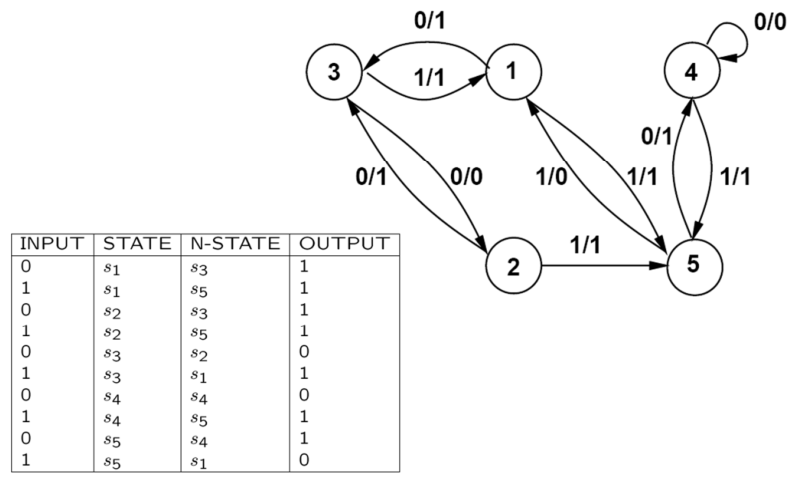
\includegraphics[height=45 mm]{./Cap2/Images/Image06.png}
	\caption[Optional caption]{State transition table and state transition diagram}
	\label{fig:stateDia}
\end{figure}

\subsubsection{Dataflow graphs – DFG (Architectural-level)}
We consider here models that abstract the information represented by procedural HDLs. Abstract models of behavior at the architectural level are in terms of  \textit{operations}  (Vertices)  and their  \textit{dependencies} (Edges).
\begin{figure}[H]
	\centering
	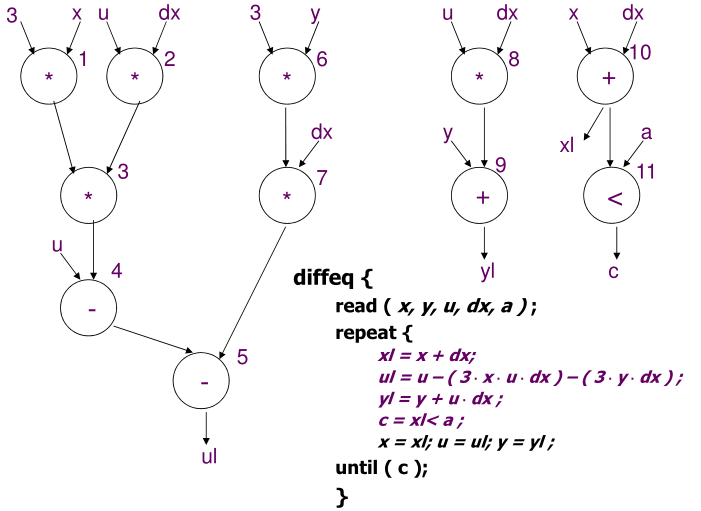
\includegraphics[height=45 mm]{./Cap2/Images/Image08.png}
	\caption[Optional caption]{DFG}
	\label{fig:DFG}
\end{figure}
Control-flow information, related to  \textit{branching}  (or  \textit{conditional})  and  \textit{iteration} (or  \textit{loop})  constructs, can also be represented graphically. Many different models have been proposed to represent \textit{control/data-flow graphs}.\\
The simplest approach is to extend further data-flow graphs by introducing branching vertices that represent operations that evaluate conditional clauses.  A  \textit{branching} vertex is the tail of a set of alternative paths, corresponding to the possible branches. \textit{Iteration} can be modelled as a branch based on the iteration exit condition. The corresponding vertex is the tail of two edges, one modelling the exit from the loop and the other the return to the first operation in the loop.\\
One particular abstract model for tasks subject to data- and control-flow dependencies is called \textit{sequencing graph}. It is a hierarchical control/data-flow graph, where control-flow primitives such as branching and iteration are modelled through the hierarchy, whereas data-flow and serialization dependencies are modelled by graphs. In addition, the hierarchical model supports a  model call,  i.e., the encapsulation of subsets of operations and their dependencies into blocks that can be multiply invoked.\\
The graph has two major properties:
\begin{itemize}
\item Acyclic
\item Polar: there are two vertices, called  \textit{source}  and  \textit{sink},  that represent the first and last tasks.
\end{itemize}
\begin{figure}[H]
    \centering
    \begin{subfigure}[b]{0.2\textwidth}
        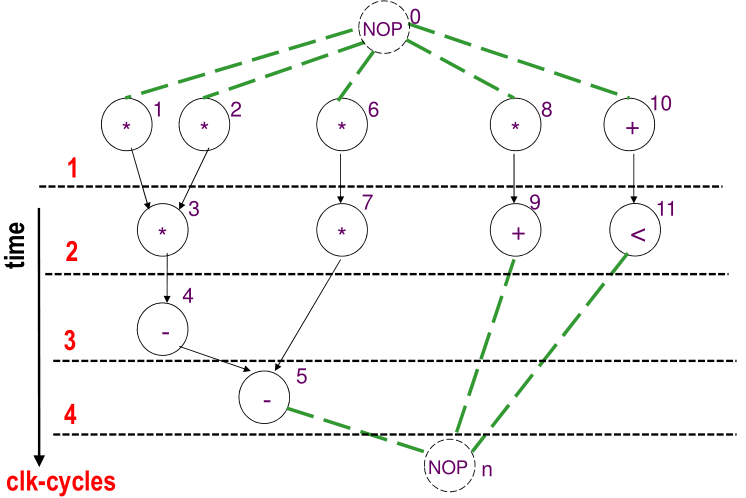
\includegraphics[width=\textwidth]{./Cap2/Images/Image09.png}
        \caption{Sequencing DFG}
        \label{fig:SequencingDFG}
    \end{subfigure}
    \quad
    \begin{subfigure}[b]{0.2\textwidth}
        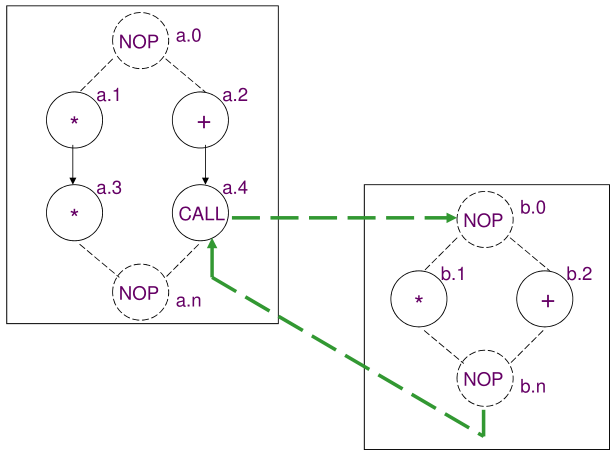
\includegraphics[width=\textwidth]{./Cap2/Images/Image10.png}
        \caption{Hierarchy DFG}
        \label{fig:HierarchyDFG}
    \end{subfigure}
    \quad
    \begin{subfigure}[b]{0.2\textwidth}
        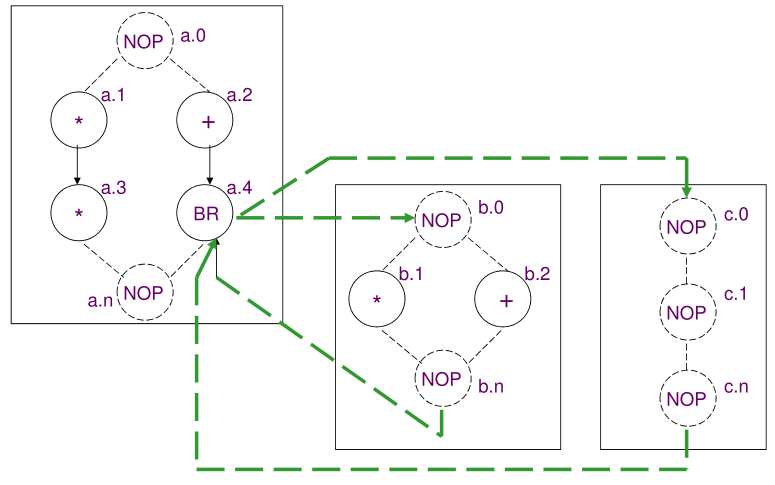
\includegraphics[width=\textwidth]{./Cap2/Images/Image11.png}
        \caption{Branching DFG}
        \label{fig:BranchingDFG}
    \end{subfigure}
    \quad
    \begin{subfigure}[b]{0.2\textwidth}
        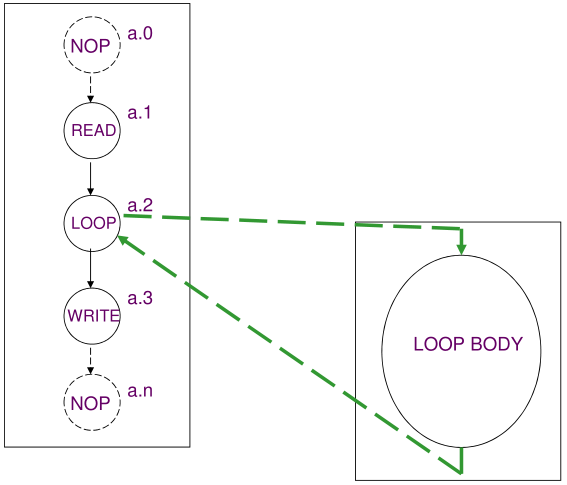
\includegraphics[width=\textwidth]{./Cap2/Images/Image12.png}
        \caption{Iteration DFG}
        \label{fig:IterationDFG}
    \end{subfigure}
    \label{fig:DFGs}
    \caption{Different examples of DFG}
\end{figure}
Some attributes can be assigned to the vertices and edges of a sequencing graph model, such as measures or estimates of the corresponding \textit{area} or delay \textit{cost}. In general, the delay of  a  vertex can be  data independent  or  data dependent.  Only data-independent delays can be estimated before synthesis. An example data-dependent iteration is given by an arithmetic divisor, based on an iterative algorithm. Data-dependent delays can be  \textit{bounded}  or  \textit{unbounded}.  The former case applies to data-dependent delay branching, where the maximum and minimum possible delays can be computed. The latter case is typical of some other iteration constructs.
\cleardoublepage
\section{Architectural-Level Synthesis}
Trying to pass from logic to architectural level racecourse at higher level allow to see all possible options. Having less details, it possible work with higher complex circuit. You can decide to use a bigger block with high complexity at logic level, but the block that you have connected and improved don't allow to see a global improvement.\\
The motivations to raise abstraction level:
\begin{itemize}
\item Reduce specification of details
\item Extend designer base
\item Ease modifications and extensions
\item Reduce design time
\item Explore and optimize macroscopic structure
\end{itemize}
Architectural synthesis means constructing the macroscopic structure of a digital circuit, starting from behavioral models that can be captured by data-flow or sequencing graphs. The outcome of architectural synthesis is both a structural view of the circuit, in particular of its data path, and a logic-level specification of its control unit. The data path is an interconnection of  \textit{resources} (implementing arithmetic or logic functions), \textit{steering logic circuits}  (e.g., multiplexers and buses), that send data to the appropriate destination at the appropriate time and  \textit{registers}  or  \textit{memory arrays}  to store data.
\begin{figure}[H]
	 \centering
	 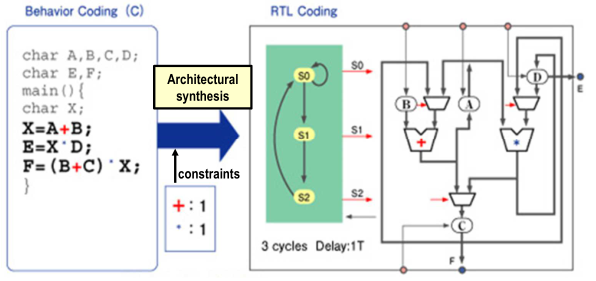
\includegraphics[height=50mm]{./Cap3/Images/Image01.png}
	 \caption[Optional caption]{Example of Architectural synthesis}
	 \label{fig:archSy}
\end{figure}

\subsection{Hardware and software compilation}
A \textit{software} compiler consists of a  front end  that transforms a program into an intermediate form  and a  back end  that translates the intermediate form into the machine code for a given architecture. The front end is language dependent, and the back end varies according to the target machine. Similarly, a \textit{hardware} compiler can be seen as consisting of a front end, an optimizer and a back end (Figure 3.16). The back end is much more complex than a software compiler, because of the requirements on timing and interface of the internal
operations.
\begin{figure}[H]
	 \centering
	 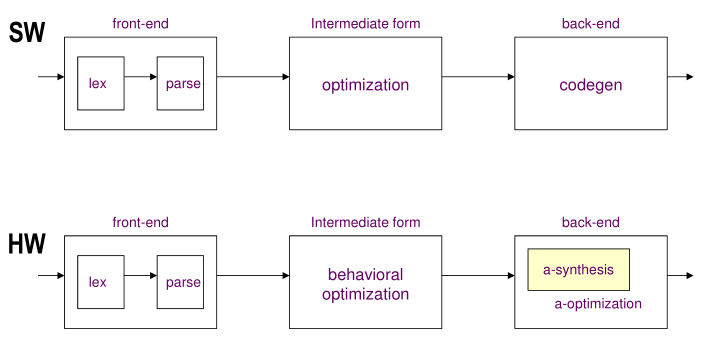
\includegraphics[height=50mm]{./Cap3/Images/Image02.png}
	 \caption[Optional caption]{Hardware and software compilation}
	 \label{fig:comp}
\end{figure}

\subsubsection{Compilation  Techniques}
The front end of a compiler is responsible for  \textit{lexical}  and  \textit{syntax} analysis, \textit{parsing}  and \textit{creation} of the intermediate form. Its first task is to verify that they satisfy the syntax rules of the language. The parser has knowledge of the grammar of the language and it generates a set of  parse trees.  A parse tree is a tree-like representation of the syntactic structure of a language. An example is shown in Figure \ref{fig:parseTree}. Syntactic errors, as well as some semantic errors are detected at this stage.
\begin{figure}[H]
	 \centering
	 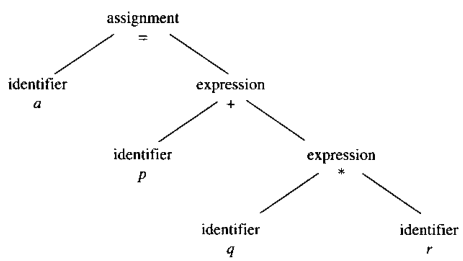
\includegraphics[height=50mm]{./Cap3/Images/Image03.png}
	 \caption[Optional caption]{Example  of  a  parse  tree  for  the statement  $ a  =  p  +  y  *  r $}
	 \label{fig:parseTree}
\end{figure}
Branching constructs can be used to model logic networks. A common way to exploit branching is by means of conditional assignments to a variable.  A  branching construct can be replaced by one logic expression, representing the disjunction of the possible assignments in conjunction with the test on the clause. When the branching construct does not specify an assignment for all values of the clause, the missing assignments represent  \textit{don't  care}  conditions on that variable. The compilation of hardware models at the architectural level involves a full \textit{semantic}, \textit{analyses}  that comprises  \textit{data-flow}  and  \textit{control-flow}  analyses.
\begin{figure}[H]
	 \centering
	 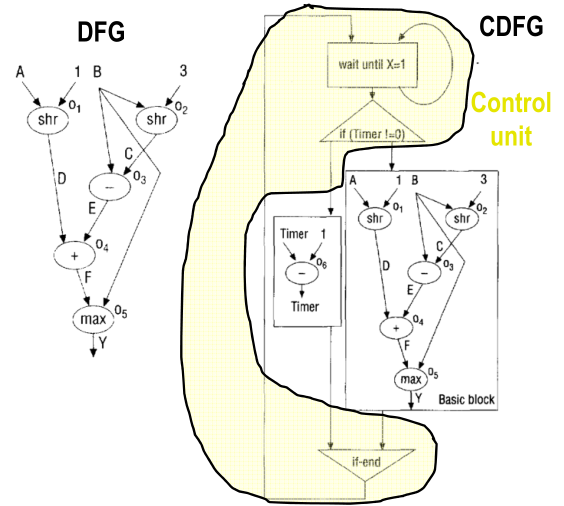
\includegraphics[height=50mm]{./Cap3/Images/Image04.png}
	 \caption[Optional caption]{Data-flow graph and Control-data-flow graph}
	 \label{fig:dataFlow}
\end{figure}

\subsubsection{Optimization Techniques}
Behavioral optimization is a set of transformations that minimize the amount of information needed to specify the partial order of tasks. It can be applied directly to the parse trees, or during the generation of the intermediate form.\\
Algorithms for behavioral optimization of  HDL  models can he classified as data-flow and control-flow
oriented.
\begin{itemize}
\item \textbf{DATA-FLOW-BASED TRANSFORMATIONS}: 
	\begin{itemize}
	\item \textit{Tree-height reduction}: This transformation applies to the arithmetic expression trees and strives to achieve the expression split into two-operand expressions, so that the parallelism available in hardware can be exploited at best. The simplest reduction algorithm uses the \textit{commutativity} and \textit{associativity} of the addition and multiplication. It permutes the operands to achieve subexpressions involving the same operator, which can be reduced by using the associative property. A  further refinement can be achieved by exploiting the \textit{distributive} property, possibly at the expense of adding an operation.
	\begin{figure}[H]
    \centering
    \begin{subfigure}[b]{0.4\textwidth}
        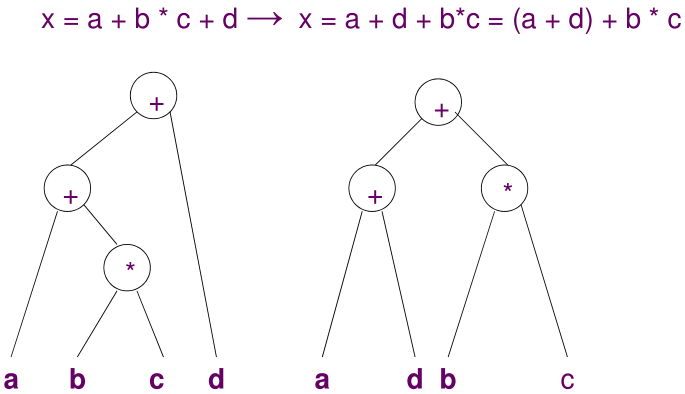
\includegraphics[width=\textwidth]{./Cap3/Images/Image05.png}
        \caption{using Commutativity and Associativity}
        \label{fig:comAss}
    \end{subfigure}
    \quad\quad\quad
    \begin{subfigure}[b]{0.4\textwidth}
        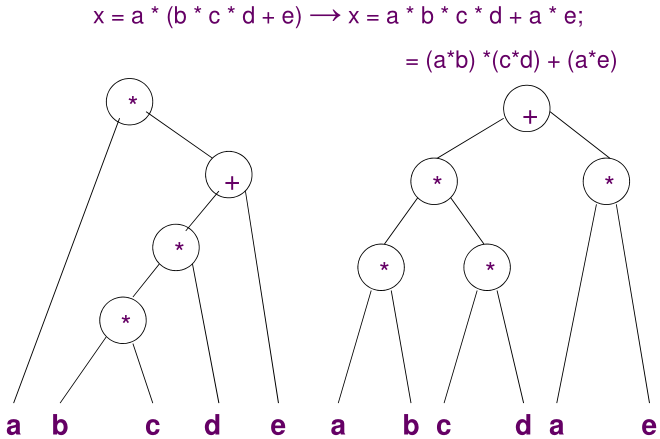
\includegraphics[width=\textwidth]{./Cap3/Images/Image06.png}
        \caption{using Distributivity}
        \label{fig:Dis}
    \end{subfigure}
	\end{figure}
	\item \textit{constant and variable propagation}:  \textit{Constant} propagation consists of detecting constant operands and pre-computing the value of the operation with that operand. Since the result may be again a constant, the new constant can be propagated to those operations that use it as input.
	\begin{figure}[H]
	 \centering
	 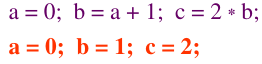
\includegraphics[width=0.25\textwidth]{./Cap3/Images/Image07.png}
	\end{figure}
	\textit{Variable} propagation consists of detecting the copies  of variables, i.e., the assignments like  x  =  y,  and using the right-hand side in the following references in place of the left-hand side. 
	\begin{figure}[H]
	 \centering
	 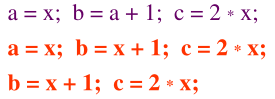
\includegraphics[width=0.25\textwidth]{./Cap3/Images/Image08.png}
	\end{figure}
	\item \textit{Common subexpression elimination}: The search for common arithmetic subexpressions relies in general on finding isomolphic patterns in the parse trees (\textit{Isomorphic}: if the subtree has the same inputs and the same operators). This step is greatly simplified if the arithmetic expressions are reduced to two-input ones. Then, this transformation consists of selecting a target arithmetic operation and searching for a preceding one of the same type and with the same operands.
	\begin{figure}[H]
	 \centering
	 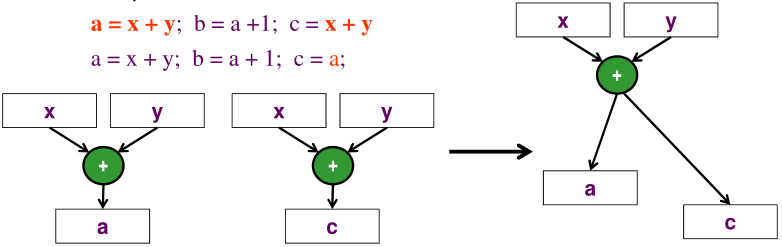
\includegraphics[width=0.4\textwidth]{./Cap3/Images/Image09.png}
	\end{figure}
	\item \textit{Dead code elimination};  Dead code consists of all those operations that cannot be reached, or whose result is never referenced elsewhere. 
	\begin{figure}[H]
	 \centering
	 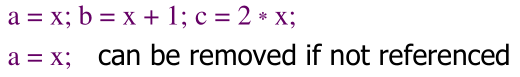
\includegraphics[width=0.4\textwidth]{./Cap3/Images/Image10.png}
	\end{figure}
	\item \textit{Operator strength reduction}:  Operator strength reduction means reducing the cost of implementing an operator by using a simpler one. 
	\begin{figure}[H]
	 \centering
	 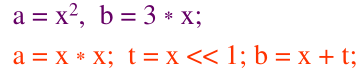
\includegraphics[width=0.3\textwidth]{./Cap3/Images/Image11.png}
	\end{figure}
	\item \textit{Code motion}:  Code motion often applies to loop invariants, i.e., quantities that are computed inside an iterative construct but whose values do not change from iteration to iteration. The goal is to avoid the repetitive evaluation of the same expression.
	\begin{figure}[H]
	 \centering
	 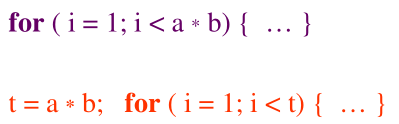
\includegraphics[width=0.3\textwidth]{./Cap3/Images/Image12.png}
	\end{figure}
	\end{itemize}
\item \textbf{CONTROL-FLOW-BASED TRANSFORMATIONS}:  The following transformations are typical of hardware compilers. In some cases these transformations are automated, in others they are user driven.
	\begin{itemize}
	\item \textit{Model expansion}: Consists in flattening locally the model call hierarchy. Therefore the called model disappears, being swallowed by the calling one. A  possible benefit is that the scope of application of some optimization techniques  is enlarged.
	\begin{figure}[H]
	 \centering
	 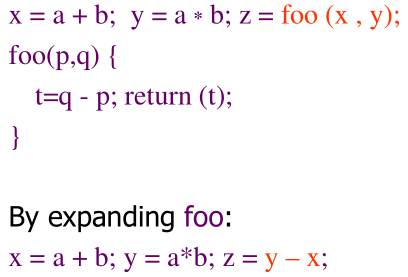
\includegraphics[width=0.3\textwidth]{./Cap3/Images/Image13.png}
	\end{figure}
	\item \textit{Conditional expansion}:  A  conditional construct can be always transformed into a parallel construct with a test in the end. Under some circumstances this transformation can increase the performance of the circuit. 
	\begin{figure}[H]
	 \centering
	 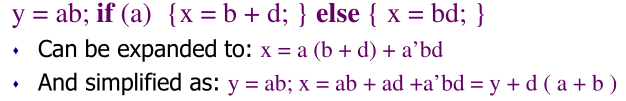
\includegraphics[width=0.5\textwidth]{./Cap3/Images/Image14.png}
	\end{figure}
	\item \textit{Loop expansion}:  Loop expansion, or unrolling, applies to an iterative construct with data-independent exit conditions. The loop is replaced by as many instances of its body as the number of operations. The benefit is again in expanding the scope of other transformations. 
	\begin{figure}[H]
	 \centering
	 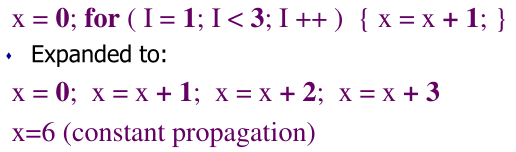
\includegraphics[width=0.4\textwidth]{./Cap3/Images/Image15.png}
	\end{figure}
	\end{itemize}
\end{itemize}

\subsection{Architectural synthesis and optimization}

\cleardoublepage
\section{Scheduling}
\begin{parsetree}
    ( .Scheduling. 
        (.Unconstrained.  `ASAP')
        (.Latency constraint.  
        	.Overall Latency.	'ACAP' $ \lambda=t_{n}-t_{0} = 5-1=4 $
        	.Detailed Latency Constraint.	$ P_{ij} \lessgtr t_{i}-t_{j} $
        	.Minimum resource under latency constraint.
        )
        (.Resource constraint.  
        	.ILP.
        	.HU'S.
        	.List Scheduling.
        )
    )
\end{parsetree}	
\cleardoublepage
\section{Resource Sharing}
\textit{Resource sharing}  is the assignment of a resource to more than one operation. The primary goal of resource sharing is to reduce the area of a circuit, by allowing multiple non-concurrent operations to share the same hardware operator. Resource sharing is often mandatory to meet specified upper bounds on the circuit area.\\
\textit{Resource  binding}  is the explicit definition of a mapping between the operations and the resources.\\
When considering \textit{resource-dominated circuits} that have been scheduled under resource constraints, the area is already determined by the resource usage. Thus binding and sharing serve just the purpose of refining the structural information so that connectivity synthesis can be performed.
\subsection{Binding/Sharing scenario}
\begin{itemize}
\item  \textbf{Dedicated resources} (min Latency, MAX Area): one resource per operation, no sharing thus Binding intrinsically defined
\item  \textbf{One multi-task resource} (Area is fixed, Latency defined by scheduling): an arithmetic co-processor that computes all necessary operations, max sharing, no binding.
\item  \textbf{One resource per type} (Area defined by sharing): there are adder, multiplier, ecc. Binding is partially defined, sharing (all operations of the same type use the same resource, the goal of the optimization problem)
\item \textbf{Many resources per type} (Area defined by binding; Sharing affected by type selection). Different types of the same operation: for the adder Ripple-carry, Carry-save, Carry-lookahead; for the multiplier Wallace, Partial Product Mult. Binding and Sharing.
\end{itemize}

\subsection{Perfect  Graphs}
Each undirected graph can be characterized by  four  numbers:
\begin{enumerate}
\item $ \omega(G) $ \textit{clique number}: the cardinality of its largest clique, called  maximum clique
\item $ K(G) $  \textit{clique cover number}: the cardinality of a minimum clique partition is equal to the cardinality of a minimum clique cover
\item $ \alpha(G) $ \textit{ stability number}: the cardinality of its largest stable set. A  stable set  is a subset of vertices with the property that no two vertices in the stable set are adjacent
\item $ \chi(G) $ \textit{chromatic number}: the cardinality of the minimum number of colors needed
to color the vertices into subsets, such that each is a stable set
\end{enumerate}
A graph is said to be  \textit{partitioned into cliques} if its vertex set is partitioned into (disjoint) subsets, each one inducing a clique. Similarly, a graph is said to be  \textit{covered} by  cliques  when the vertex set can  be  subdivided into (possibly overlapping) subsets, each one inducing a clique.\\
The size of the maximum clique is a lower bound for the chromatic number, because all vertices in that clique must be colored differently
\[ \omega(G) \leq \chi(G) \]
Similarly, the stability number is a lower bound for the clique cover number, since each vertex of the stable set must belong to a different clique of a clique cover
\[ \alpha(G) \leq K(G) \]
A graph is said to he  \textit{perfect}  when the inequalities can be replaced by equalities.
\bigskip \\
An \textit{interval graph} is a graph whose vertices can be put in one-to-one correspondence with a set of  intervals, so that two vertices are adjacent if and only if the corresponding intervals intersect.
\begin{figure}[H]
    \centering
    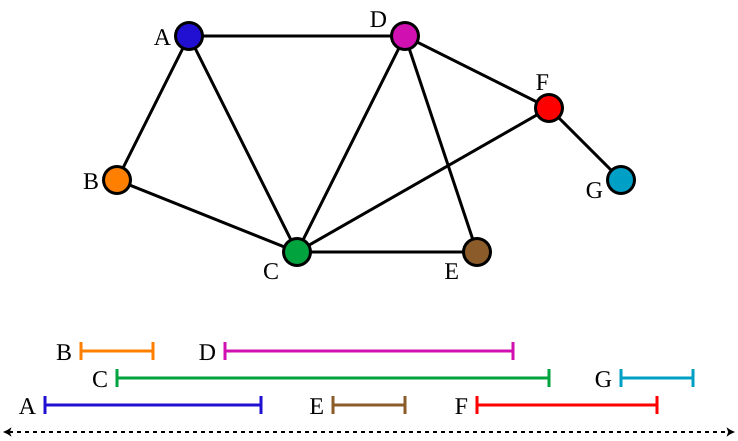
\includegraphics[width=0.45\textwidth]{./Cap5/Images/Image05.png}
    \caption{interval graph}
    \label{fig:intervalgraph}
\end{figure}
A graph  is a  \textit{comparability graph}  if it satisfies the  \textit{transitive orientation property},  i.e., if it has an orientation such that in the resulting directed graph
\[G(V,F),\:\: \lbrace (v_i,v_j)\in F\:and\: (v_j,v_k)\in F \rbrace \Rightarrow (v_i,v_k)\in F \]

\paragraph{Example}
Consider the graph of Figure \ref{fig:Undirec}a.
\begin{itemize}
\item The size of the maximum clique $ \lbrace v_1,v_2,v_3 \rbrace $ is $ \omega(G)=3 $
\item The graph can be partitioned into cliques $ \lbrace v_1,v_2,v_3 \rbrace $ and $ \lbrace v_4 \rbrace $.  Alternatively,  it  can be covered by cliques $ \lbrace v_1,v_2,v_3 \rbrace $ and $ \lbrace v_1,v_3,v_4 \rbrace $. The clique cover number $ K(G) = 2$
\item  The largest stable set is  $ \lbrace v_2,v_4 \rbrace $.  Thus, the stability number is $ \alpha(G) = 2$ 
\item  A  minimum coloring would require three colors for $ \lbrace v_1,v_2,v_3 \rbrace $. Vertex $ \lbrace v_4 \rbrace $ can have the same color as $ \lbrace v_2 \rbrace $.  Hence the chromatic number $ \chi(G)=3$.
\end{itemize}
Because $ \alpha(G) = K(G) = 2 $, the graph is perfect.\\
Figure \ref{fig:Undirec}(b) shows an orientation that does not satisfy the transitive property (because there is no edge between vertices $ v_2 $  and  $ v_4 $).  Nevertheless, the orientation shown in Figure  \ref{fig:Undirec}(c) (obtained by reversing the direction of the edge between $ v_3 $  and  $ v_4 $)  has the transitive property. Hence the graph of Figure  \ref{fig:Undirec}(a) is a comparability graph.
\begin{figure}[H]
    \centering
    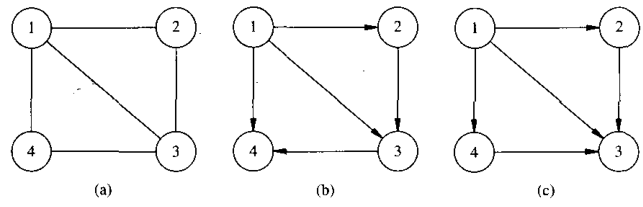
\includegraphics[width=0.45\textwidth]{./Cap5/Images/Image04.png}
    \caption{(a)  Undirected  graph.  (b)  An  orientation.  (c)  A  transitive  orienlarion.}
    \label{fig:Undirec}
\end{figure}	



\subsection{Sharing and binding for resource-dominated circuits}
We consider sharing and binding problems for resource-dominated circuits modeled by scheduled (operation concurrency well defined) sequencing graph $ G_s(V,E) $. The source and sink vertices  $ v_0,v_n $  are \textit{No-Operations}. Hence the operation set of interest is $ \lbrace v_i,i=1,2,...,n \rbrace $.\\
Two (or more) operations may be bound to the same resource if:
\begin{enumerate}
\item they are not concurrent (not used in the same time step)
\item they can  be  implemented by resources of the same type
\end{enumerate}
When these conditions are met, the operations are said to be  \textbf{compatible}.  Two operations are not concurrent when either one starts after the other has finished execution or when they are alternative.
\bigskip \\
The \textbf{resource compatibility graph} $ G_{+}(V,E) $ is a graph whose vertex set $ V = \lbrace v_i,i=1,2,...,n_{ops} \rbrace $ is in one-to-one correspondence  with  the operations and 	whose edge set $ E = \lbrace \lbrace v_i, v_j \rbrace ,i,j=1,2,...,n_{ops} \rbrace $ denotes the compatible operation pairs.
\bigskip \\
The resource compatibility graph has at least as many disjoint components as the resource types. A group of mutually compatible operations corresponds to a subset of vertices that are all mutually connected by edges, i.e., to a clique. Therefore a \textit{maximal}  set of mutually compatible operations is represented by a  maximal clique  in the compatibility graph.\\
\textbf{An  optimum resource sharing} is one that minimizes the number of required resource instances. Since we can associate a resource instance to each clique, the problem is equivalent to partitioning the graph into a minimum number of cliques. Such a number is the  \textit{clique cover number} denoted by $ K $.

\paragraph{Example}
Let us consider the scheduled sequencing graph of Figure \ref{fig:SchSeqG}. We  assume again that there are two resource types:  a  multiplier and  an  ALU,  both  with  1  unit execution delay. The compatibility graph is shown in Figure \ref{fig:Compat}. Examples of compatible operations are $ \lbrace v_1,v_3 \rbrace $ and $ \lbrace v_4,v_5 \rbrace $ among others. Examples of cliques are the sub graphs induced by $ \lbrace v_1,v_3,v_7 \rbrace $, $ \lbrace v_2,v_6,v_8 \rbrace $ and $ \lbrace v_4,v_5,v_{10},v_{11} \rbrace $.   These cliques, in addition to $ \lbrace v_9 \rbrace $,  cover the graph. Since they  are disjoint, they form a clique partition. The \textit{clique cover number} $ K $  is then equal to  4,corresponding to two multipliers and two ALUs.
\begin{figure}[H]
    \centering
    \begin{subfigure}[b]{0.45\textwidth}
        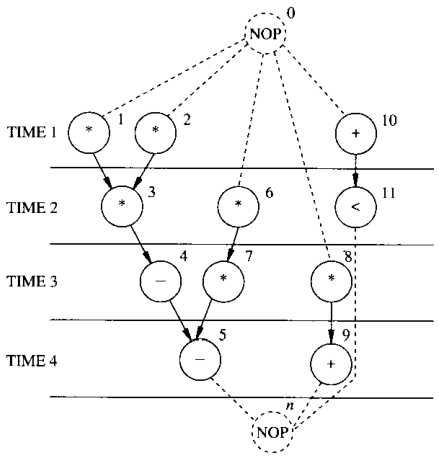
\includegraphics[width=\textwidth]{./Cap5/Images/Image01.png}
        \caption{Scheduled  sequencing  graph}
   		\label{fig:SchSeqG}
    \end{subfigure}
    \quad\quad\quad
    \begin{subfigure}[b]{0.45\textwidth}
        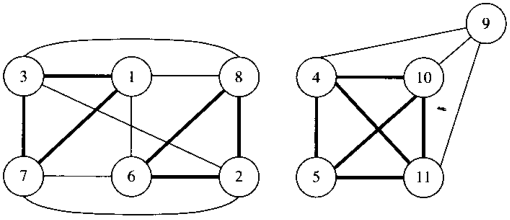
\includegraphics[width=\textwidth]{./Cap5/Images/Image02.png}
        \caption{Compatibility graph of the multiplier and the ALU types}
   		\label{fig:Compat}
    \end{subfigure}
    \caption{}
\end{figure}
An alternative way of looking at the problem is to consider the  conflicts  between operation pairs. Two operations have a conflict when they are not compatible. Conflicts can be represented by  conflict graphs.
\bigskip \\
The \textbf{resource conflict graph} $ G_{-}(V,E) $ is a graph whose vertex set $ V = \lbrace v_i,i=1,2,...,n_{ops} \rbrace $ is in one-to-one correspondence  with  the operations and 	whose edge set $ E = \lbrace \lbrace v_i, v_j \rbrace ,i,j=1,2,...,n_{ops} \rbrace $ denotes  the conflicting operation pairs.
\bigskip \\
A  proper vertex coloring of the conflict graph provides a solution to the sharing problem: each color corresponds to a resource instance. All vertexes connected must have different colors.\\
\textbf{An optimum resource sharing} corresponds to a vertex coloring with a minimum number of colors. Such a number is the  \textit{chromatic number} denoted by $ \chi $.  Note that $ K= \chi $

\paragraph{Example}
Consider again the scheduled sequencing graph of Figure \ref{fig:SchSeqG}. We show in Figure  \ref{fig:ConfGr}  the conflict graphs for the multiplier and  ALU  types. Examples of independent sets are   among others. Each graph  can  he colored with two colors, yielding an overall resource requirement of  4.
\begin{figure}[H]
    \centering
    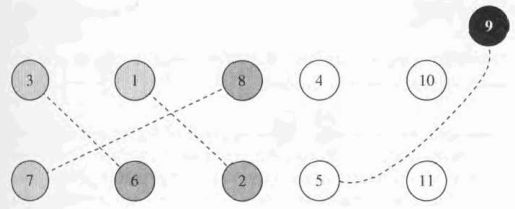
\includegraphics[width=0.45\textwidth]{./Cap5/Images/Image03.png}
    \caption{Conflict  graphs  for  the  multiplier  and  ALU  types}
    \label{fig:ConfGr}
\end{figure}	
Exact and heuristic solution methods have been proposed to solve the \textit{clique partitioning} and \textit{vertex coloring} problems.


\subsection{Resource Sharing}
Two operations are compatible  if  they can be implemented by resources of the same type and if they are not concurrent. Therefore, the \textit{compatibility graph} $ G_{+}(V,E) $ is described by the a set of edges that connect two operations of the same operation type and have different start time. Such a graph can be constructed by traversing the sequencing graph. This graph is a \textit{comparability graph} because it has a transitive orientation property. Indeed, a corresponding directed graph could be derived by assigning an orientation to the edge.
\begin{figure}[H]
    \centering
    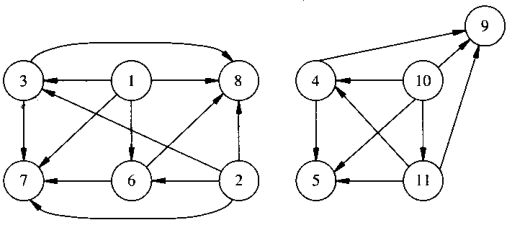
\includegraphics[width=0.45\textwidth]{./Cap5/Images/Image06.png}
    \caption{Transitive  orientation  of  the compatibility  graph for the multiplier and for the ALU types}
    \label{fig:Transi}
\end{figure}

Let us consider now the \textit{conflict graphs} for each resource type. Vertices correspond to  intervals  and  e edges correspond to interval intersection. Hence they are \textit{interval graphs}. The search for a minimum coloring of an interval graph can be achieved in polynomial time.  A  few algorithms can  be  used, including the Golumbic’s algorithm and \textit{LEFT-EDGE}  algorithm.
\begin{figure}[H]
    \centering
    \begin{subfigure}[b]{0.2\textwidth}
        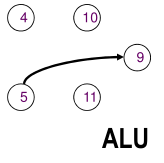
\includegraphics[width=\textwidth]{./Cap5/Images/Image09.png}
        \caption{}
   		\label{fig:mul}
    \end{subfigure}
    \quad\quad\quad
    \begin{subfigure}[b]{0.2\textwidth}
        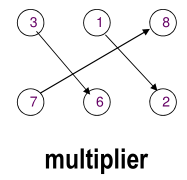
\includegraphics[width=\textwidth]{./Cap5/Images/Image08.png}
        \caption{}
   		\label{fig:alu}
    \end{subfigure}
    \quad\quad\quad
    \begin{subfigure}[b]{0.45\textwidth}
        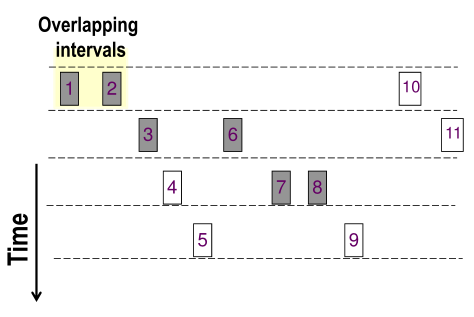
\includegraphics[width=\textwidth]{./Cap5/Images/Image07.png}
        \caption{Overlapping intervals}
   		\label{fig:Overlapping intervals}
    \end{subfigure}
    \caption{}
\end{figure}

\paragraph{Left-Edge Algorithm}
is a coloring algorithm applied on an inteval graph. This algorithm takes as input the set of intervals with \textit{left and right edge} and a set of \textit{colors} (initially one). The principles of the algorithm are the following ones:
\begin{enumerate}
	\item Sort the invervals in a \textit{list} by the \textit{left} edge
	\item Assing non overlapping interval to the forst color according with the \textit{sorted list}.
	\item When epossible intevals are exhausted, increase color and repeat.
\end{enumerate}
\begin{figure}[H]
	\centering$  $
	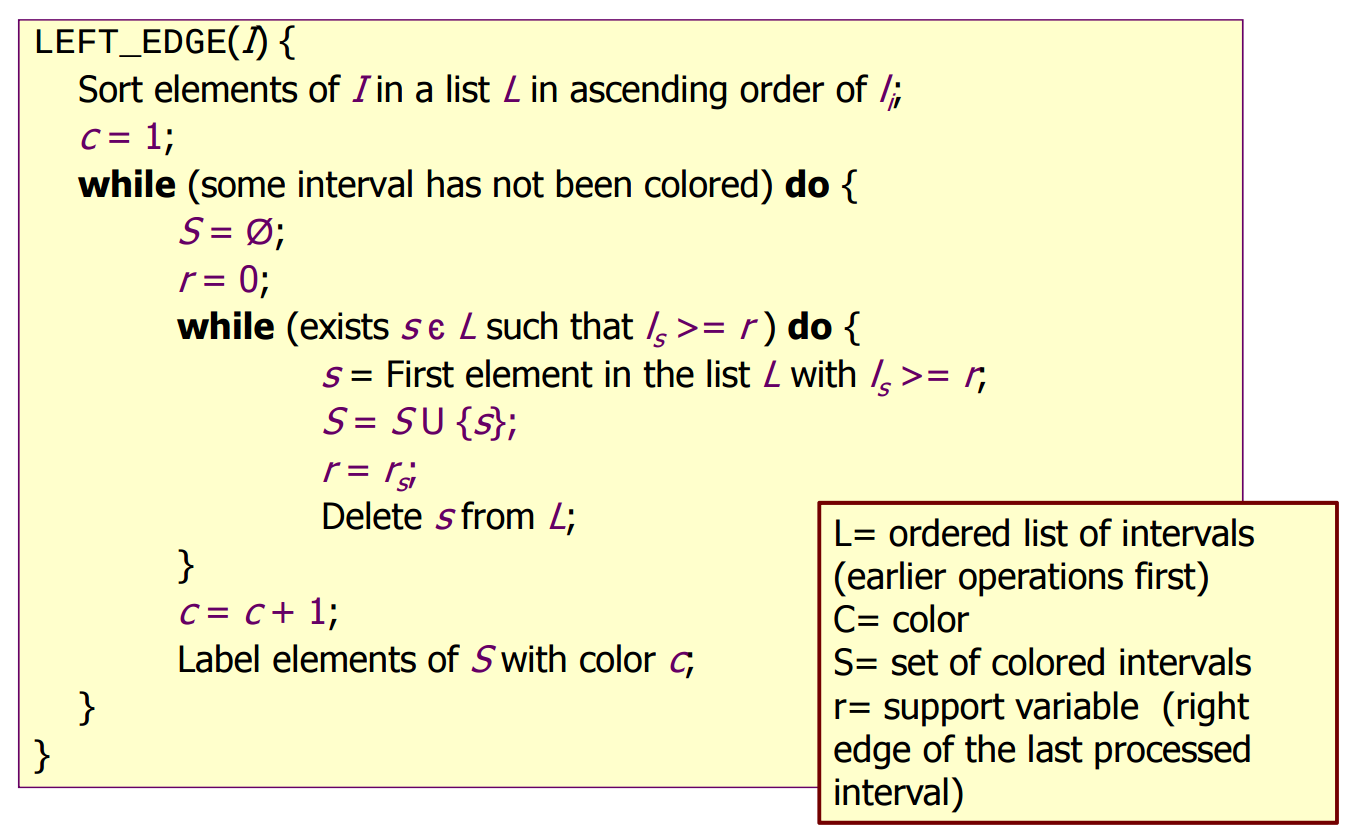
\includegraphics[width=0.60\textwidth]{./Cap5/Images/Image10.png}
	\caption{Pseudo-Code of Left-Edge algorithm}
	\label{fig:PseudoLEalg}
\end{figure}
\begin{figure}[H]
	\centering
	\begin{subfigure}[b]{0.19\textwidth}
		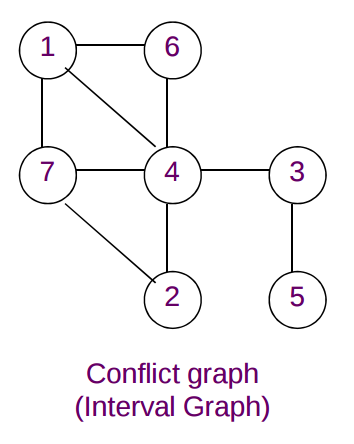
\includegraphics[width=\textwidth]{./Cap5/Images/Image11.png}
		\caption{}
		\label{fig:conflGraph}
	\end{subfigure}
	\quad\quad\quad
	\begin{subfigure}[b]{0.19\textwidth}
		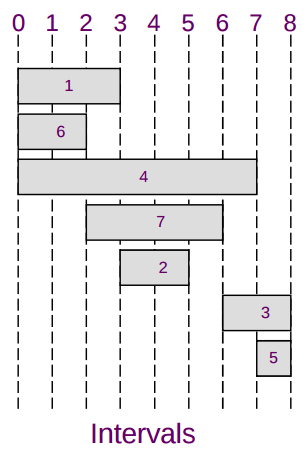
\includegraphics[width=\textwidth]{./Cap5/Images/Image12.png}
		\caption{}
		\label{fig:intervalsLE}
	\end{subfigure}
	\quad\quad\quad
	\begin{subfigure}[b]{0.2\textwidth}
		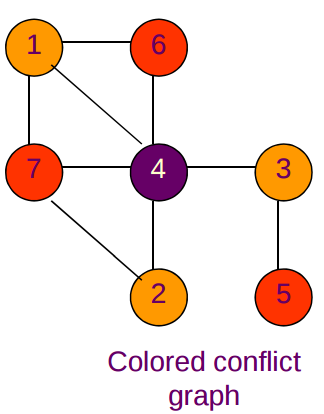
\includegraphics[width=\textwidth]{./Cap5/Images/Image13.png}
		\caption{}
		\label{fig:coloredConflict}
	\end{subfigure}
	\begin{subfigure}[b]{0.2\textwidth}
		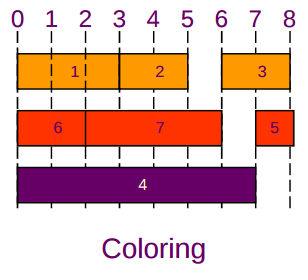
\includegraphics[width=\textwidth]{./Cap5/Images/Image14.png}
		\caption{}
		\label{fig:coloring}
	\end{subfigure}
	\caption{}
\end{figure}
\subsection{Register Sharing}
Registers are used to hold values of variables and to share them we have to consider their \textit{lifetime} (interval between the generation and the last reference of a variable). Variables that are alive in different intervals or under alternative conditions can share the same register. Such variables are called \textit{compatible}
\bigskip\\
Starting from a schedule and assuming that variables with multiple assignment are aliased, we can derive the lifetime of each variables and build a \textit{Conflict Graph} similar to previous ones but this time: 
\begin{enumerate}
	\item Vertices $\longleftrightarrow$ variables.
	\item Edges $\longleftrightarrow$ Overlaps (between variables lifetime)
\end{enumerate}
Next, we can build the \textbf{Compatibility} Graph that complement the conflict graph and show us.
\paragraph{Algorithm: }
Starting from a lifetime conflict graph, our goal is to find the \textit{minimum} number of registers storing all the variables. To reach this goal we can use the \textit{Left-Edge algorithm} (polynomial complexity) but if there are iterative conflict (some variables are alive across the iteration boundary) coloring problem is intractable, so we have to use heuristic algorithms.
\subsection{Bus Sharing and Binding}
Busses act as transfer resources that feed data to functional resources. The operation of writing a specific bus can be modeled explicitly as a vertex in the sequencing graph model. In this case, the compatible (or conflicting) data transfers may be represented by compatibility (or conflict) graphs, as in the case of functional resources.
\bigskip\\
Two problems then arise:
\begin{enumerate}
	\item Find the minimum number of busses to accommodate all (or part of) the data transfers
	\item Find the maximum number of
	data transfers that can be done through a given number of busses.
\end{enumerate}
These problems are analogous to the multi-port binding problem and can be modeled by \textit{ILP constraints}.
\subsection{Module Selection Problem}
The resource-type selection problem, called also module selection, is a \textit{generalization of the binding problem}, where we assume that more than one resource type can match the functional requirements of an operation type. We say that two resource types are \textbf{compatible} if they can perform the same operation. An example is given by the addition operation and the resource types corresponding to \textit{ripple-carry} and \textit{carry look-ahead} adders. Both resource types fulfill the required functionality, but with different area and propagation delay that are the decision variables for this type of problem.
\bigskip\\
Several \textit{heuristic methods} have been proposed for the module selection problem. When a minimum-latency schedule is the goal, the fastest resource types are used in scheduling. Resource sharing and module selection are then applied to minimize the area, in that case slower and smaller resources can be assigned to non-critical operations.

\paragraph{Data path synthesis}
is applied after resource binding and produce: the connection of resources to \textit{multiplexers busses and registers}, interface towards control unit and \textit{I/O ports}.

\begin{figure}[H]
	\centering
	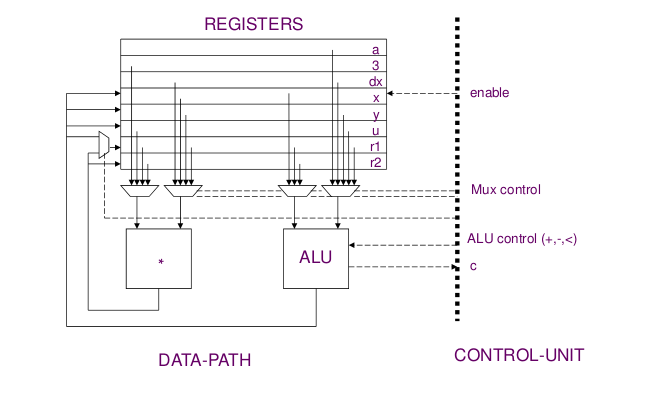
\includegraphics[width=0.50\textwidth]{./Cap5/Images/Image15.png}
	\caption{Example of Data path synthesis}
	\label{fig:dpsynth}
\end{figure}

\paragraph{Control synthesis}
is referred to the synthesis of the control unit starting from scheduling model and obtaining a \textit{syncronous FSM}. The phisical implementation of the control unit can be done with \textit{Hard wired FSM} 
\begin{itemize}
	\item \textit{Hard wired} FSM 
	\item Memory-based Microcode (programmable)
\end{itemize} 

\begin{figure}[H]
	\centering
	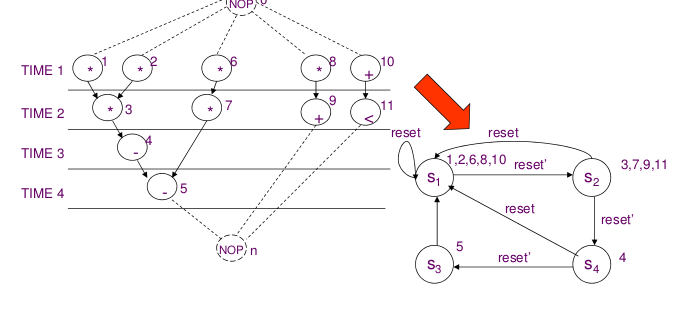
\includegraphics[width=0.60\textwidth]{./Cap5/Images/Image16.png}
	\caption{Example of Control synthesis}
	\label{fig:contrsynth}
\end{figure}

\begin{figure}[H]
	\centering
	\begin{subfigure}[b]{0.30\textwidth}
		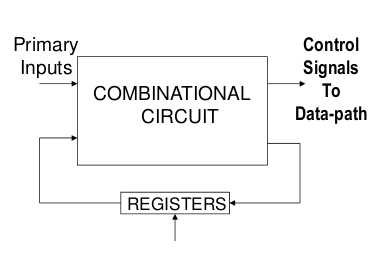
\includegraphics[width=\textwidth]{./Cap5/Images/Image17.png}
		\caption{}
		\label{fig:hardWiredCU}
	\end{subfigure}
	\quad\quad\quad
	\begin{subfigure}[b]{0.30\textwidth}
		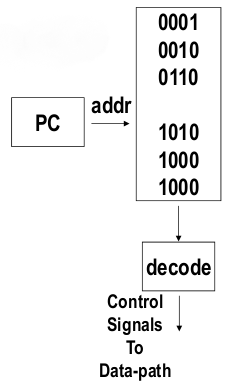
\includegraphics[width=\textwidth]{./Cap5/Images/Image18.png}
		\caption{}
		\label{fig:programCU}
	\end{subfigure}
	\caption{Possible Implementation of Control Unit}
\end{figure}

\cleardoublepage
\section{Two Level Logic Synthesis Optimization}
We distinguish between sequential and combinational circuits, whose behaviour can be captured by finite-state machine state diagrams or by Boolean functions and relations. Often, sequential and combinational circuits are represented conveniently by mixed structural/behavioural models, such as  \textit{logic networks}. The goal of logic-level synthesis and optimization is to determine the microscopic structure of a circuit, i.e., its gate-level representation. \\
This chapter deals with the optimization of combinational logic circuits, modeled by two-level  \textit{sum of products}  expression forms.	
\bigskip\\
The \textbf{objective} of two-level synthesis optimization are:
\begin{itemize}
	\item Minimization of the area
	\item Optimization of performance(\textit{I/O delay} for combinational circuits and \textit{register to register path} for sequential circuit).
	\item Minimize power consumption
\end{itemize}
\bigskip
To implement a given funztion we have different possibilities, infact, in this example we can obtain different value for area and delay.\\
Given $ f = pqrs $ we obtain (a) (b) (c) (d) as possible implementations:
\begin{figure}[H]
	\centering
	\begin{subfigure}[b]{0.5\textwidth}
		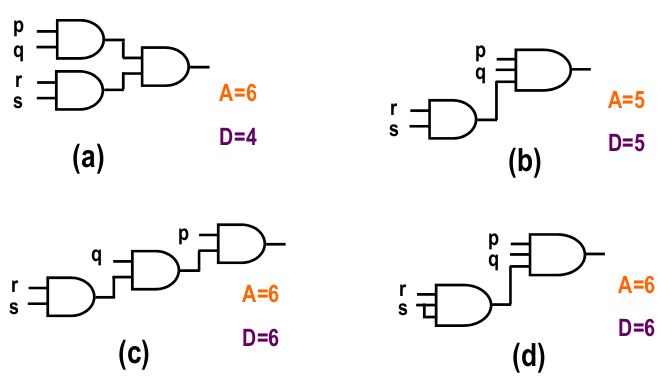
\includegraphics[width=\textwidth]{./Cap6/Images/Image1.png}
		\caption{Different Implementation}
		\label{fig:possImpl}
	\end{subfigure}
	\quad\quad
	\begin{subfigure}[b]{0.4\textwidth}
		\includegraphics[width=\textwidth]{./Cap6/Images/Image2.png}
		\caption{Performance comparison}
		\label{fig:perform}
	\end{subfigure}
\end{figure}
In this case only (a) and (b) are part of pareto points, and they achieve different goal, in area or delay.

\subsection{Background and Definitions}
The \textbf{Boolean functions} we use in this case are:
\begin{itemize}
	\item \textit{Binary} Input and Output $ B = \{0, 1\} $ 
	\item \textit{Single} ( $ f : B^{n} \rightarrow B $ ) or\textit{ Multiple} (  $ f : B^{n} \rightarrow B^{m} $ ) output
	\item \textbf{Incompletely specified} so, functions \underline{with} don't care conditions ($ f: B^{n} = \{0, 1, *\} $)
\end{itemize}
\paragraph{Don't care condition}
The case in which we don't care about the value of a function, it's r\textit{related to the evirnonment} (input pattern that never occours or input patter for which some output is never observed),
\paragraph{ON-set}
Subset of the domain that make $ f = true $
\paragraph{OFF-set}
Subset of the domain that make $ f = false $
\paragraph{DC-set}
Subset of the domain for which we observe a \textit{don't care} value
\bigskip\\
For \textit{multiple output function}  ON, OFF and DC set is defined \textit{for each} component
\bigskip\\
We can give different representation that can be summarized into two categories: \textbf{visual} (Karnaugh Maps, Truth Table, Cubical Notation) or \textbf{computer oriented} (Matrices, BDDs) representations.
\begin{figure}[H]
	\centering
	\includegraphics[width=0.6\textwidth]{./Cap6/Images/Image3.png}
	\caption{Cubical representation, in which each vertex of the cube is a minterm, can associate positional value. Example: $ ab'c \rightarrow 1_{a}0_{b}1_{c} $ \textit{(1 indicates true value)}}
	\label{fig:cubicalnotation}
\end{figure}
\paragraph{Definitions}
\begin{itemize}
	\item Boolean \textbf{variables} (\textit{Example: a, b, c, ...}) 
	\item Boolean \textbf{literals} are variables and their complement ( \textit{Example: a, a', b, b', ...})
	\item \textbf{Product or cube} is a product of literals (\textit{Example: ab'c, b'c, ...})
	\item A \textbf{Minterm} is product of \textit{all input variables} and implies a value for the function (usually 1)
	\item \textbf{Implicant} is a product (\textit{not mandatory to contain all the input variables}) that implies a value for the function (usually 1)
\end{itemize}
\paragraph{Tabular Representation}: define a truth ttable with the list of all minterm of a given function, and define a \textbf{cover} also called \textbf{implicant table} that is a list of all the implicant sufficient to define the function (\textit{Note}: implicant table is generally smaller in size than the truth table of the same function)

\begin{center}
	
	\begin{tabular}{|c|c|}
		\hline
		abc & xy \\ \hline
		000 & 00 \\ \hline
		001 & 10 \\ \hline
		010 & 00 \\ \hline
		011 & 11 \\ \hline
		100 & 00 \\ \hline
		101 & 01 \\ \hline
		110 & 11 \\ \hline
		111 & 11 \\ \hline 
	\end{tabular}
	\quad
	\quad
	\quad
	\quad
	\quad
	\quad
	\quad
	\begin{tabular}{|c|c|}
		\hline
		abc & xy \\ \hline
		001 & 10 \\ \hline
		*11 & 11 \\ \hline
		101 & 01 \\ \hline
		11* & 11 \\ \hline 
	\end{tabular}
	
	\bigskip
	Complete \textit{truth table} for $ x= ab + a'c $ and $ y = ab + bc+ ac $ (left side) and \textit{implicant table} (right side)
\end{center}
\paragraph{Logic Synthesis Problem} are related to the \textbf{implementation styles} (PLA macro-cells for \textit{two level circuits} and cell/array based for \textit{multi-level circuits}) and to the \textbf{operation mode} of the circuit (combinational, syncronous sequential or asyncronous sequential).

\subsection{Optimization for two-level circuits}
The reason why we invest so much time to the two level logic optimization are:

\begin{itemize}
	\item \textbf{Reduction} in the size of the representation
	\item \textbf{Direct implementation} of standard operating procedures (PLAs reduce size and delay).
	\item \textbf{implementation styles} based on Multi-Level nets
\end{itemize}

\subsubsection{Programmable Logic Arrays}
PLas are macro-cells with rectangular structure that implement any multi-output function. Their layout is generated by module generators and it's very popular in the '70/'80 but they are still used in some modern application, such as smart controllers, and in emerging technologies (Graphene, Crossbar Latch). They have some \textbf{advantages} as simplicity and predictable timing, but also the \textbf{disadvantages} of not much flexibility (with respect to cell based realization)
\paragraph{Graphene PLAs} are an open topic for researcher because there are interesting features of the graphene that allow us to recreate a complex function with a very low usage of gates (and so better performance and less area utilization)

\subsubsection{Approaches of Two-level Optimization}
Assuming that all implicants have the same cost, our goals are, the \textit{reduction of the number of implicants and literals}, infact implicants correspond to a PLA rows and literals to transistors.

\paragraph{Minimum cover} is the cover of a function with the \textit{minimum} number of implicants (\textbf{Global Optimum})

\paragraph{Minimal or irreduntant cover} is a cover that isn't a superset of another one (\textit{no implicant can be dropped}) and correspond to \textbf{local optimum}.

\paragraph{Minimal with respect to 1 implicant containment} cover in which no implicant is contained by another one (\textbf{weak local optimum})

Given this definition we can use \textit{exact methods} to compute \textit{\underline{minimum cover}} (often difficult/impossible for large function) or \textit{\underline{}} to compute \textit{\underline{minimal cover}}

\begin{itemize}
	\item \textbf{Exact Methods} are based on Quine's theorem (Quine-McCluskey, Petrick's methos, Espresso exact)
	\item \textbf{Heuristic Methods} MINI, PRESTO, ESPRESSO and so on.
\end{itemize}
Considering all possible implicant, we define some subset with some characteristics:
\begin{itemize}
	\item \textbf{Prime implicant}, implicant \textit{not} contained or covered by any other implicant
	\item \textbf{Prime cover} a cover in which \textit{all} implicants are prime
	\item \textbf{Essential Prime implicants} covers a minterm \textit{not} covered by any one else. They \textit{needs} to be included into the cover 
\end{itemize}
\subsubsection{Exact Logic Minimization}
The most used algorithms are based on \textit{Quine's theorem} that says:
\begin{center}
	\textit{There is a minimum cover that is prime}\\
\end{center}
and as consequence of this theorem we restrict our search of minimum cover only to prime implicants; for this reason the Quine-Based methods:
\begin{enumerate}
	\item Compute the prime implicants
	\item Determine the minimum cover
\end{enumerate} 
All the exact methods need the\textit{ primes table as starting point}, so that the optimization problem is reduced to a covering problem.\\
Considering a completely specified single-output functions, a \textbf{prime implicant table} is a binary-valued matrix $A$ whose columns are in one-to-one correspondence with the prime implicants of the function $f$ and whose rows are in one-to-one correspondence with its minterms.\\ 
A minimum cover is a minimum set of columns which covers all rows, or equivalently a minimum set of primes covering all minterms. Therefore the covering problem can be viewed as the problem of finding a binary vector $x$ representing a set of primes with minimum cardinality $|x|$ such that:
\begin{center}
	$Ax \geqslant \textbf{1}$
\end{center}
where \textbf{1} is the "unary vector" and as $x$ match he number of minterms and primes.

\paragraph{Example} given the function $ f= a'b'c' + a'b'c + ab'c + abc + abc' $

\begin{center}
	
	\begin{tabular}{|c|c|c|}
		\hline
		$\alpha$ & 00* & 1 \\ \hline
		$\beta$ & *01 & 1 \\ \hline
		$\gamma$ & 1*1 & 1 \\ \hline
		$\delta$ & 11* & 1 \\ \hline
	
	\end{tabular}
	\quad
	\quad
	\quad
	\quad
	\begin{tabular}{|c|c c c c|}
		\hline
		 {} & $\alpha$ & $\beta$ & $\gamma$ & $\delta$ \\ \hline
		 000 & 1 & 0 & 0 & 0 \\ \hline
		 001 & 1 & 1 & 0 & 0 \\ \hline
		 101 & 0 & 1 & 1 & 0 \\ \hline
		 111 & 0 & 0 & 1 & 1 \\ \hline
		 110 & 0 & 0 & 0 & 1 \\ \hline
		 
	\end{tabular}

	\bigskip
	
	\textit{Primes} to the left side, \textit{Prime table} to the right side
\end{center}

Then use the $x$ vector multiplied by $A$ to compute if all the implicant are covered, so:

\begin{center}
	
	\begin{tabular}{ c c }
	
		\begin{tabular}{|c c c c|}
			
			1 & 0 & 0 & 0 \\
			1 & 1 & 0 & 0 \\ 
			0 & 1 & 1 & 0 \\ 
			0 & 0 & 1 & 1 \\ 
			0 & 0 & 0 & 1 \\ 

			
		\end{tabular}
		
	\quad
	\quad
	
		\begin{tabular}{|c|}
			
			$x_{\alpha}$ \\
			$x_{\beta}$ \\
			$x_{\gamma}$ \\
			$x_{\delta}$ \\
			
		\end{tabular}
		
	\end{tabular}
	\bigskip
	
	Assigning to $x_{\alpha}, x_{\beta} ... $ value 1 only if it's considered part of the cover, then try to remove one of them from the cover and recompute if $Ax \geqslant \textbf{1}$, repeat this until find the \textit{minimum cover}.
\end{center}
\paragraph{Covering Problem} is a \underline{NP-hard problem} due to:
\begin{itemize}
	\item Columns - prime implicants (Up to $3^{n}/3$)
	\item Rows - minterms ($2^{n}$).
	\item Selection Boolean vector for primes $x$ and determine it such that $Ax \geqslant \textbf{1}$ 
	\item Select at the same time \textit{enough columns} to cover all rows and \textit{minimize the cardinality} of $x$.
\end{itemize}
\subsection{Quine-McCluskey}
The method involves two steps:
\begin{enumerate}
	\item Finding all prime implicants of the function.
	\item Use those prime implicants in a prime implicant chart to find the essential prime implicants of the function, as well as other prime implicants that are necessary to cover the function.
\end{enumerate} 
\paragraph{Example} Given the function $ f(x,y,z,v) = \Sigma m(1,4,5,6,7,9,11,14,15) $ so that the function will be equal to 1 for the values specified (1,4,5,6...), in the following step we attempt reduction and merge some minterms wher their \textit{mindistance  = 1}

\begin{center}
  
\begin{tabular}{ c c }
	
	\begin{tabular}{|c c c c|c c|}
		\hline
		x & y & z & v & res & val \\ \hline
		0 & 0 & 0 & 0 & 0 & {} \\ 
		0 & 0 & 0 & 1 & 1 & \textbf{m1} \\
		0 & 0 & 1 & 0 & 0 & {} \\
		0 & 0 & 1 & 1 & 0 & {} \\
		0 & 1 & 0 & 0 & 1 & \textbf{m4} \\
		0 & 1 & 0 & 1 & 1 & \textbf{m5} \\
		0 & 1 & 1 & 0 & 1 & \textbf{m6} \\
		0 & 1 & 1 & 1 & 1 & \textbf{m7} \\
		1 & 0 & 0 & 0 & 0 & {} \\
		1 & 0 & 0 & 1 & 1 & \textbf{m9} \\
		1 & 0 & 1 & 0 & 0 & {} \\
		1 & 0 & 1 & 1 & 1 & \textbf{m11} \\
		1 & 1 & 0 & 0 & 0 & {} \\
		1 & 1 & 0 & 1 & 0 & {} \\
		1 & 1 & 1 & 0 & 1 & \textbf{m15} \\	
		1 & 1 & 1 & 1 & 1 & \textbf{m14} \\ \hline
	\end{tabular}
	
	\quad
	\quad
	\quad
	
	\begin{tabular}{|c c c c c |c|}
		\hline
		{} & x & y & z & v & {} \\ \hline
		m1 & 0 & 0 & 0 & 1 & \checkmark \\ 
		m4 & 0 & 1 & 0 & 0 & \checkmark  \\
		m5 & 0 & 1 & 0 & 1 & \checkmark  \\
		m6 & 0 & 1 & 1 & 0 & \checkmark  \\
		m7 & 1 & 1 & 1 & 1 & \checkmark  \\
		m9 & 1 & 0 & 0 & 1 & \checkmark  \\
		m11 & 1 & 0 & 1 & 1 & \checkmark  \\
		m14 & 1 & 1 & 1 & 0 & \checkmark   \\
		m15 & 1 & 1 & 1 & 1 & \checkmark  \\ \hline
		
		
	\end{tabular}
	
	\quad
	\quad
	\quad
	
	\begin{tabular}{|c c c c c |c|}
		\hline
		
		{} & x & y & z & v & {} \\ \hline
		m1-m5 & 0 & * & 0 & 1 & \textbf{a} \\ 
		m1-m4 & * & 0 & 0 & 1 & \textbf{b}  \\
		m4-m5 & 0 & 1 & 0 & * & \checkmark  \\
		m4-m6 & 0 & 1 & * & 0 & \checkmark  \\
		m5-m7 & 0 & 1 & * & 1 & \checkmark  \\
		m6-m7 & 0 & 1 & 1 & * & \checkmark  \\
		m6-m14 & * & 1 & 1 & 0 & \checkmark  \\
		m7-m15 & * & 1 & 1 & 1 & \checkmark   \\
		m9-m11 & 1 & 0 & * & 1 & \textbf{c}  \\
		m11-m15 & 1 & 1 & 1 & * & \checkmark  \\ 
		m14-m15 & 1 & * & 1 & 1 & \textbf{d}  \\ \hline
		
	\end{tabular}
	
	\end{tabular}
	

	
	\begin{tabular}{|c c c c c |c|}
		\hline
		
		{} & x & y & z & v & {} \\ \hline
		m4-m5-m6-m7 & 0 & 1 & * & * & \textbf{e} \\ 
		m6-m7-m14-m15 & * & 1 & 1 & * & \textbf{f}  \\ \hline
		
	\end{tabular}

\end{center}
\bigskip
In this case \textbf{a, b, c, d, e, f} are implicant included into the cover because cannot be merged.\\
Now we have to identify the \textbf{essential prime implicants} and include it into the cover. To identify the essential we have to check if that implicant is the only one that cover \textit{a minterm}, in that case it's essential and has to be part of the cover.





\begin{center}
	
	\begin{tabular}{|c| c c c c c c|}
		\hline
		{} & a & b & c & d & \textbf{e} & \textbf{f} \\ \hline
		m1 & 1 & 1 & {} & {} & {} & {} \\
		m4 & {} & {} & {} & {} & \underline{\textbf{1}} & {} \\
		m5 & 1 & {} & {} & {} & 1 & {} \\
		m6 & {} & {} & {} & {} & 1 & 1 \\
		m7 & {} & {} & {} & {} & 1 & 1 \\
		m9 & {} & 1 & 1 & {} & {} & {} \\
		m11 & {} & {} & 1 & 1 & {} & {} \\
		m14 & {} & {} & {} & {} & {} & \underline{\textbf{1}} \\
		m15 & {} & {} & {} & 1 & {} & {} \\ \hline
		
	\end{tabular}
	
\bigskip
In this case \textit{e and f} are essential because they are the only that covers m4 (covered by e) and m14 (covered by f). Selecting these two implicans we have to consider all the minterms covered already by these. After that we can chose the prime implicants that are not essential. The only minterms that remain uncovered are: m1, m9, m11.

	\begin{tabular}{|c| c c c c |}
		\hline
		{} & a & \textbf{b} & \textbf{c} & d  \\ \hline
		m1 & 1 & 1 & {} & {} \\
		m9 & {} & 1 & 1 & {} \\
		m11 & {} & {} & 1 & 1 \\ \hline
	
	\end{tabular}
\bigskip

The final cover will be \textbf{ e, f, b, c } so that $f = yz + x'y + y'z'v + xy'v$ 

\end{center}

\subsection{Petrick's Method}





	
\end{document}